\chapter{深度伪造与检测的背景}
\label{chap:1}
近年来人工智能与深度学习等计算机学科的蓬勃发展,连带也造成的不同研究领域与多样的议题需要进行研讨,比如讨论在以人工智慧应有的社会治理架构下,讨论其机器学习领域等演算法等对于法学所造成的挑战\cite{law01},同时另一篇研究也讨论其人工智能与演算法在法律上应用的可能 \cite{law03}。而在机器学习领域下的深度伪造技术则发展有越来越广泛的趋势,而其深度伪造属于机器学习下的深度学习的一部分,而深度学习已经广泛应用于各个领域,其领域包含了计算机视觉与自然语言处理,而本作业则关注当中快速兴起的则是深度伪造的领域,其深度伪造技术\cite{list1101}虽造成了风险,但同时在这些年也有需多研究去分析深度伪造的工作原理,并且引入了许多基于深度学习的方法来检测深度伪造的影像或图像。

综上所述这些技术好的部分则是应用于将古老的照片变成动态的影像,或者是用于一些艺术与网路次文化的创作,又或者是 Reface APP\cite{list1102} 等服务带给大众娱乐,但同时负面的因素也有造成社会动荡的可能,包含知名人士被伪造影像、近而被广泛散布不实资讯与谣言的危险,造成当事人的声誉、社会地位与事业严重打击,还有近期大量知名女姓人士被用于成人色情网站,而受害当事人却因执法基层人员不理解相对应技术亦或是没有完善的检测工具,因而在此方面无法给予有效的协助,而受害人在描述其受害过程时受到再次的心理创伤,同时其深度伪造的假影片在网路散布时,对当事人的伤害就已经造成。再者此技术近期被应用在战争宣传战,将敌对方的政治人物伪造出用于其不正确的政治发言影片,进而造成某方的士气遭到打击。

\begin{figure}[htb]
\centering 
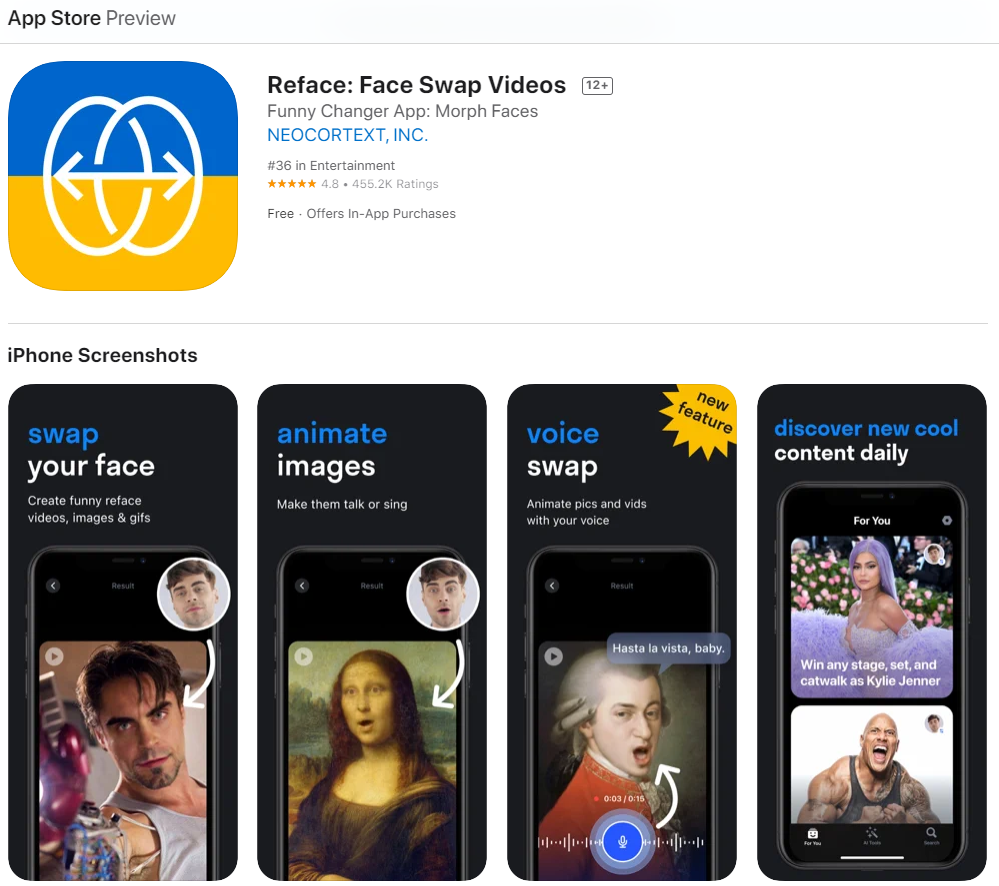
\includegraphics[width=0.50\textwidth]{img/ch1m1.png} 
\caption{Reface APP 苹果商店页面}
\label{Test}
\end{figure}

另外需要注意的在于这些工具非常容易取得,与之相应的是一些相继机构发现这些问题后,进而举办相应的竞赛\cite{list1103},来推广该技术在此领域的热度。所以本作业即目标即探讨在人工智能下的深度学习领域中深度伪造与其检测的研究整理,同时调研过去Girish N 等人所汇整的早期图像篡改工作 \cite{girish2019review}与 Nguyen TT 等人 对该领域工作地早期总结 \cite{nguyen2019deep}与 Li XR 等人近期来的汇整工作\cite{2021496} 与研读,同时对使用深度学习方法下深度伪造与相对应的前沿检测技术进行调查,并对目前最新的研究进行补充。

\section{深度伪造技术}

目前对深度伪造技术在视觉上所修改后的影像与图片,其大多是针对人类脸部的替换。而在此大致分为两大部分,其一为对人类的人脸表情进行伪造,让指定窜改者所改造的对象做到窜改者想要的脸部表情与动作,但不对该人脸进行目标人脸的替换,另一类则是根据两个不同影像与影片的人脸进行替换,经过将另一个完全不同身份的人脸替换过去,从而达到该内容目标人物是窜改者所要之人。该技术从过往运用的三维重建技术等方法来修改之外,一路发展到运用深度学习的方法至今则用生成对抗网路为基础进行仿造,比如 Almars, A. M 等人在该领域工作汇整之一的 CycleGAN,此方法为无监督方法,它提取一张图像的特征,并通过 GAN 架构生成另一张具有相同特征的图像。该方法应用循环损失函数,使他们能够学习潜在特征,且该方法应用循环损失函数,使他们能够学习潜在特征,可以在不使用配对示例的情况下执行图像到图像的转换。换句话说,该模型从源和目标中学习不需要相互关联的图像集合的特征。而更重要的是目前的仿造技术还运用人类语音的修改,从而导致伪造出来的影像结果会更逼真。

\begin{figure}[htb]
\centering 
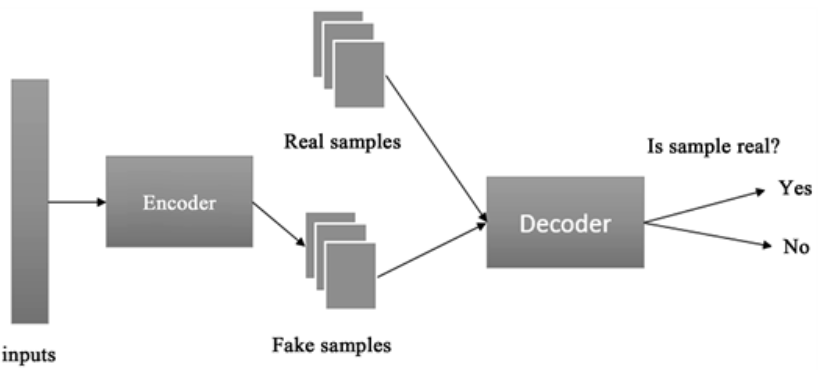
\includegraphics[width=0.80\textwidth]{img/ch1m2.png} 
\caption{Almars, A. M 等人整理的 GAN 深度伪造示意}
\label{Test}
\end{figure}

\subsection{针对人类脸部的伪造技术}

\subsubsection{过往根据图形学所进行的脸部伪造技术}

在过往几年来使用图形学来对人类的脸部进行替换和仿造的技术,一直被很多研究者持续的关注,而在 Zollhöfer M 等人对其领域进行调研总结的工作则说明地当下几个主要根据三维模型重建与追踪再该领域技术上的应用。该研究将讨论重点放在中心任务是使用基于优化的重建算法来恢复和跟踪人脸的三维模型的方法上,同时对现实世界图像形成的基本概念进行了深入的概述,并讨论了使这些算法实用的常见假设和简化。此外,该研究广泛涵盖了用于更好地约束欠约束单目重建问题的先验,并讨论了用于从单目 2D 数据中恢复密集的照片几何 3D 人脸模型的优化技术。最后,在动作捕捉、面部动画以及图像和视频编辑的背景下讨论了所审查算法的各种用例。

而 FaceSwap \cite{list1107} 是一个根据图形学的人脸替换方法,该应用是 Marek Kowalski 于华沙理工大学就读多媒体数学时,所做的练习成果,其应用程序是用 Python 编写的,并使用人脸对齐、高斯牛顿优化和图像混合来将相机看到的人脸与提供的图像中的人脸交换。同时该应用的新版本则基于深度对齐网络方法,如果在 GPU 上运行,它比当前使用的方法更快,并且提供更稳定和更精确的面部标志。另外 Dale K 等人\cite{dale2011video}提出了一种替换视频中人类脸部的方法,该研究的方法考虑了源视频和目标视频之间在身份、视觉外观、语音和时间方面的差异。该研究与以前的工作不同,它不需要大量的手动操作或复杂的采集硬件,只需要单机视频,研究者使用 3D 多线性模型来跟踪两个视频中的面部表现,使用相应的 3D 几何,最后将源扭曲到目标面并重新定时源以匹配目标性能。然后,研究者通过视频体积计算最佳接缝,以保持最终合成中的时间一致性。

\begin{figure}[htb]
\centering 
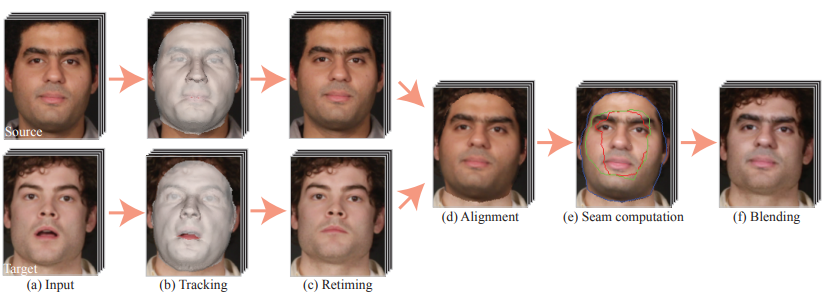
\includegraphics[width=0.80\textwidth]{img/ch1m3.png} 
\caption{Dale K 等人一种基于图像的面部重建系统}
\label{Test}
\end{figure}

Garrido P \cite{garrido2014automatic} 等人则研究提出了一种基于图像的面部重建系统,该系统将现有目标视频中的演员面部替换为源视频中用户的面部,同时保留原始目标表现,其系统是全自动的,不需要源表达式数据库。相反,它能够从使用现成相机(例如网络摄像头)捕获的短源视频中产生令人信服的重演结果,用户在其中执行任意的面部表情,研究者的重演流程被设想为部分图像检索和部分面部转移:图像检索基于目标帧的时间聚类和一种新颖的图像匹配度量,该度量结合了外观和运动以从源视频中选择候选帧,而面部转移使用保留用户身份的 2D 变形策略。其系统在简单性方面表现出色,因为它不依赖于 3D 人脸模型,它在头部运动下很稳健,并且不需要源和目标性能相似。

\begin{figure}[htb]
\centering 
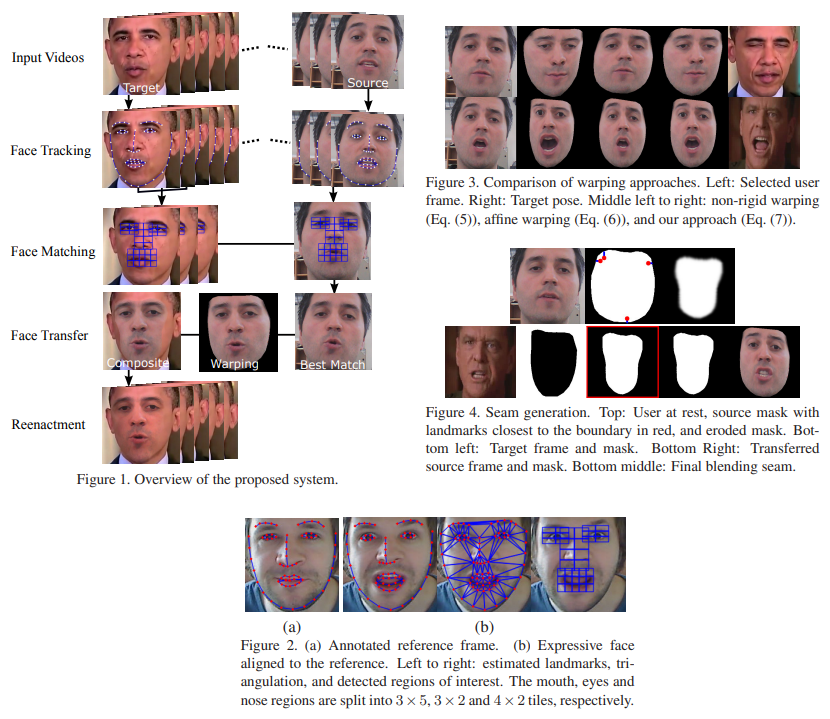
\includegraphics[width=0.80\textwidth]{img/ch1m4.png} 
\caption{Garrido P 等人一种基于图像的面部重建系统}
\label{Test}
\end{figure}

同样也是 Garrido P 等人\cite{garrido2015vdub},考虑到在许多国家,外国电影和电视作品被配音,即演员的原声被配音演员用该国自己的语言所说的翻译代替,配音是一个复杂的过程,需要特定的翻译和准确定时的朗诵,以使新音频至少粗略地贴合视频中的嘴巴动作。然而,由于原作和配音语言中的音素和视位序列不同,视频与音频的匹配永远不会完美,这是视觉不适的主要来源,在本文中,研究者提出了一种系统来改变视频中演员的嘴部动作,使其与新的音轨相匹配。其研究建立在对配音和目标演员的 3D 面部表演、照明和反照率的高质量单目捕捉的基础上,并结合使用音频分析和时空检索方法来合成一个新的照片般逼真的渲染和高度详细的 3D 形状嘴区域模型来替换目标性能。

\begin{figure}[htb]
\centering 
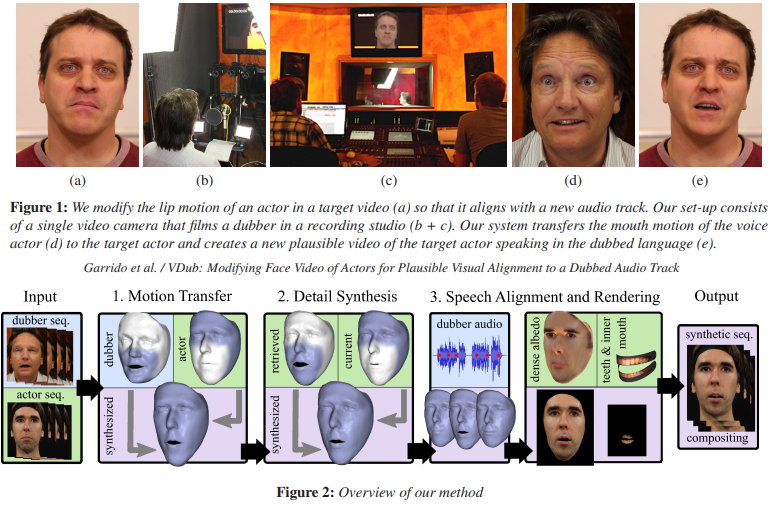
\includegraphics[width=0.80\textwidth]{img/ch1m5.png} 
\caption{Garrido P 等人提出了一种系统来改变视频中演员的嘴部动作,使其与新的音轨相匹配}
\label{Test}
\end{figure}

而 Nirkin Y 等人\cite{nirkin2018face}的研究让我们知道即使人脸图像不受约束且任意配对,它们之间的人脸交换实际上也非常简单。为此,该研究做出以下贡献。 (a) 没有像其他人之前提出的那样为人脸分割定制系统,而是展示了标准的全卷积网络 (FCN) 可以实现非常快速和准确的分割,前提是它在足够丰富的示例集上进行训练。为此,描述了新的数据收集和生成例程,这些例程提供了具有挑战性的分割人脸示例。 (b) 使用该研究的分割在前所未有的条件下实现强大的面部交换。 (c) 与以前的工作不同,该研究的交换足够强大,可以进行广泛的定量测试。为此,研究者使用野外标记人脸 (LFW) 基准测试并测量对象内和对象间人脸交换对识别的影响。研究表明,其受试者内部交换的面孔仍然与其来源一样可识别,证明了我们方法的有效性。与众所周知的感知研究一致,而更好的面部交换会产生不太可识别的主体间结果。这是第一次在机器视觉系统中定量证明这种效果。

\begin{figure}[htb]
\centering 
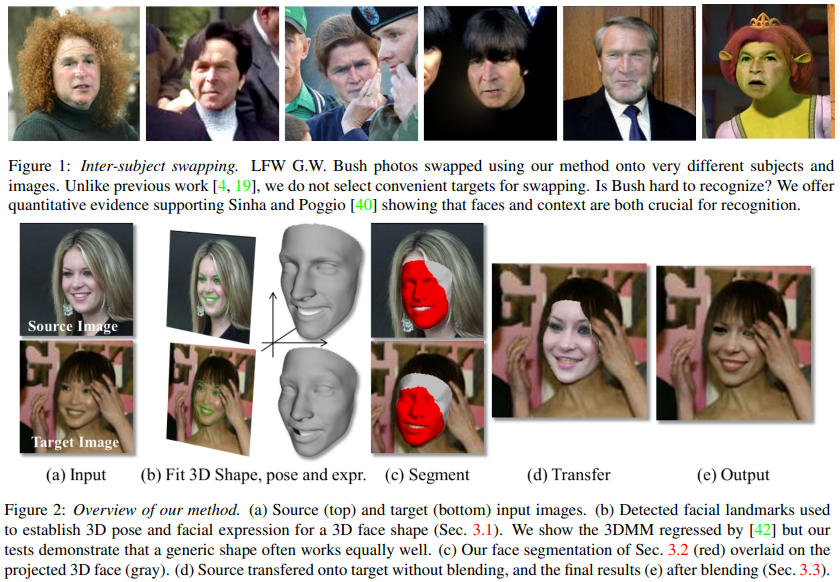
\includegraphics[width=0.80\textwidth]{img/ch1m6.png} 
\caption{Nirkin Y 用分割的思路促进换脸}
\label{Test}
\end{figure}

\subsubsection{现在根据深度学习所进行的脸部伪造技术}

由于过往图形学在面对伪造人类脸部技术有着极大的成本等诸多因素,从而导致该技术很难普遍的进行应用。然而自进入人工智能与机器学习所带动的深度学习热潮下,深度伪造技术在此之后有着非常快速的进展,此时许多研究者们开始关心其深度学习在人类脸部进行替换等应用技术。比如 Lu Z 等人 \cite{lu2017recent}则该研究领域所涉及传统方法和高级深度学习方法的典型人脸合成工作进行了全面回顾。特别是,Generative Adversarial Net (GAN) 被突出显示以生成照片般逼真和身份保持的结果。此外,还详细介绍了公开可用的数据库和评估指标。

当中 FaceSwap \cite{list1101} 是较早的一种利用深度学习来识别和交换图片和视频中的人脸的工具的 GitHub 开源项目,为具有多平台 Deepfakes 软件,其技术由 Tensorflow、Keras 和 Python 提供支持,并在 Windows、macOS 和 Linux 上运行。该原理为

\begin{figure}[htb]
\centering 
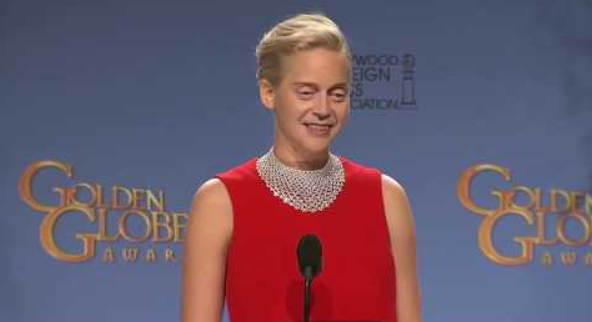
\includegraphics[width=0.80\textwidth]{img/ch1m7.png} 
\caption{FaceSwap 的 Jennifer Lawrence/Steve Buscemi FaceSwap using the Villain model}
\label{Test}
\end{figure}



%\begin{itemize}
%\item [-][7,7] 空间卷积到 1*1*2048 然后一维卷积到 1*1*128
%\item [-]池化层到 1*1*2048 然后一维卷积到 1*1*128
%\end{itemize}



%\begin{itemize}
%\item Calculus
%\item Linear Algebra
%\item Basic Computer Concepts
%\end{itemize}

%\begin{description}
% \item[First] \hfill \\
% The first item
% \item[Second] \hfill \\
% The second item
% \item[Third] \hfill \\
% The third etc \ldots
%\end{description}
